\documentclass[10pt,twocolumn,letterpaper]{article}

\usepackage{cvpr}
\usepackage{times}
\usepackage{epsfig}
\usepackage{graphicx}
\usepackage{amsmath}
\usepackage{amssymb}

% Include other packages here, before hyperref.

% If you comment hyperref and then uncomment it, you should delete
% egpaper.aux before re-running latex.  (Or just hit 'q' on the first latex
% run, let it finish, and you should be clear).
\usepackage[breaklinks=true,bookmarks=false]{hyperref}

\cvprfinalcopy % *** Uncomment this line for the final submission

\def\cvprPaperID{****} % *** Enter the CVPR Paper ID here
\def\httilde{\mbox{\tt\raisebox{-.5ex}{\symbol{126}}}}

% Pages are numbered in submission mode, and unnumbered in camera-ready
%\ifcvprfinal\pagestyle{empty}\fi
% \setcounter{page}{4321}
\begin{document}

%%%%%%%%% TITLE
\title{2020 Fall COMP4471 Project Final Report\\Google Landmark Recognition}

\author{LAM Man Hei\\
HKUST\\
{\tt\small mhlamaf@ust.hk}
% For a paper whose authors are all at the same institution,
% omit the following lines up until the closing ``}''.
% Additional authors and addresses can be added with ``\and'',
% just like the second author.
% To save space, use either the email address or home page, not both
\and
LIAO Yi Han\\
HKUST\\
{\tt\small yliaoag@ust.hk}
}

\maketitle
%\thispagestyle{empty}

%%%%%%%%% ABSTRACT
\begin{abstract}
    Deep convolution neural network has already gotten remarkable results in image classification tasks in recent years. Therefore, in this project, we will attempt to construct a landmark recognition model with deep convolution neural network to recognize the specific landmark in an image. ResNet\cite{he_deep_2015} and EfficientNet\cite{tan_efficientnet_2020} with label-distribution-aware margin loss \cite{cao_learning_2019}, which is used to mitigate to effect of imbalanced dataset, have been tested and evaluated. Also, multiple approaches are applied, including transfer learning and mixed-precision training, in order to reduce the training and inference time. From the experiment result, although both models perform similarly, we decided EfficientNet is a better recognition model over ResNet due to parameter size difference.
\end{abstract}

%%%%%%%%% BODY TEXT
\section{Introduction}

Landmark recognition can be very useful in our daily life. For instance, \href{https://www.google.com/imghp}{Google Image Search} allows users to search similar images by uploading an image instead of normal text search, but it can only search images with similar style or context. The search engine cannot recognize the landmark in the image and then provide similar images from the same landmark. This also happens in photo management service, such as Google Photo, which can only identify general objects in photos, but not the specific landmark in the photo. If the service can recognize the landmark in the uploaded photos, users can better manage their photo collection by categorizing their photos by locations. It is especially helpful for photos without location information.

In this project, we are going to investigate landmark recognition with deep convolution neural network. We will attempt to use ResNet\cite{he_deep_2015} and EfficientNet\cite{tan_efficientnet_2020} to construct a landmark recognition model. The expected output of the model is a column vector of the probability of each label. The label with the highest probability would be the predicted label of that image. Both model performance will be evaluated with some basic metrics, such as accuracy, F1-score and confusion matrix, and the best model will be elected as the final landmark recognition model.

After experiments, ResNet and EfficientNet both obtain similar performance with the accuracy of 67.70\% and 68.19\%, and average F1 score of 0.60 and 0.61 respectively. The majority classes mostly achieve great performance, but many minority classes do not perform well.

%------------------------------------------------------------------------
\section{Related Work}
\paragraph{ResNet.} ResNet \cite{he_deep_2015} is a image classification model first proposed in 2015, and won the first prize of ILSVRC 2015 \cite{ILSVRC15}. ResNet is built with a CNN architecture shown in figure \ref{fig:resnet_block}, which is based on the concept of residual learning. Shortcut connections are added in between convolution layers in the ResNet building block. This architecture resolves the degradation problem of very deep convolution neural network \cite{he_deep_2015}, and thus ResNet can achieve high accuracy by stacking over 100 convolution layers.

\begin{figure}
    \centering
    \includegraphics[width=0.35\textwidth]{img/ResNet building blocks.png}
    \caption{ResNet Building Block \cite{he_deep_2015}}
    \label{fig:resnet_block}
\end{figure}

\paragraph{EfficientNet.} EfficientNet \cite{tan_efficientnet_2020} provide a new model scaling method for CNN architectures which uses simple yet effective compound coefficient to scale up CNNs. It uniformly scales each dimension (such as width, depth, and resolution) with a fixed set of scaling coefficients. The baseline network of EfficientNet uses mobile inverted bottleneck convolution (MBConv) shown in figure \ref{fig:efficientnet_conv}. EfficientNet model can achieve high accuracy and better efficiency over other CNN models with reduced parameter size.

\begin{figure}
    \centering
    \includegraphics[width=0.35\textwidth]{COMP4471_Final_Report/img/MBConv.png}
    \caption{EfficientNet Mobile Inverted Bottleneck Conv \cite{tan_efficientnet_2020}}
    \label{fig:efficientnet_conv}
\end{figure}

\paragraph{Dataset Resampling.} Data imbalance is a common issue for the real-world dataset, yet deep neural network performs very bad in imbalanced dataset \cite{buda_systematic_2018} and have difficulties in learning representation of minority class. Thus, resampling is used to convert an imbalanced dataset into a balanced dataset. Random oversampling and undersampling are two of the common resampling techniques. However, random oversampling can lead to overfitting problem \cite{chawla_smote_2002} since the algorithm just duplicates the samples of minority classes. SMOTE \cite{chawla_smote_2002} is a more advanced oversampling algorithm to overcome the overfitting issue, which creates new samples by interpolating neighboring samples. Although undersampling is preferable to oversampling in some cases, undersampling has a significant drawback that a large portion of majority class samples will be discarded. In general, resampling is not suitable to construct a balanced dataset from a severely imbalanced dataset.

\paragraph{LDAM Loss.} Label-distribution-aware margin loss \cite{cao_learning_2019} is another method to resolve data imbalance issue, which aims to have the optimal trade-off between margins of each class, which encourages the minority classes to have larger margins like figure \ref{fig:ldam_magin}, as a large margin can be regarded as regularization. It proposes to improve the generalization error of minority classes via regularizing the minority classes more strongly and at the same time keep the model's ability to fit the frequent classes.

\begin{figure}
    \centering
    \includegraphics[width=0.35\textwidth]{COMP4471_Final_Report/img/ldam_margin.png}
    \caption{LDAM Customized Margin\cite{}}
    \label{fig:ldam_magin}
\end{figure}

%------------------------------------------------------------------------
\section{Data}
The dataset used in this project is retrieved from Google Landmark Recognition 2020\footnote{\url{www.kaggle.com/c/landmark-recognition-2020}}, which is a Kaggle competition. Since the competition is closed and no longer accept submission, the ground truth of the test dataset cannot be retrieved. Thus, only the train dataset will be used in this project. The entire dataset consists of 81313 landmarks classes with 1580470 images.

\subsection{Exploratory Data Analysis}
In exploratory data analysis (EDA), we inspect the dataset and summarize the following characteristics of the dataset.

First, the dataset is severely imbalanced. The largest landmark class has a sample size of 6272 while the smallest landmark class only has a sample size of 2. Almost 97.5\% of the landmark classes are with sample size under 100. The frequency graph in figure \ref{fig:dist_data} can clearly show that there are very few classes having a large sample size.

\begin{figure}
    \centering
    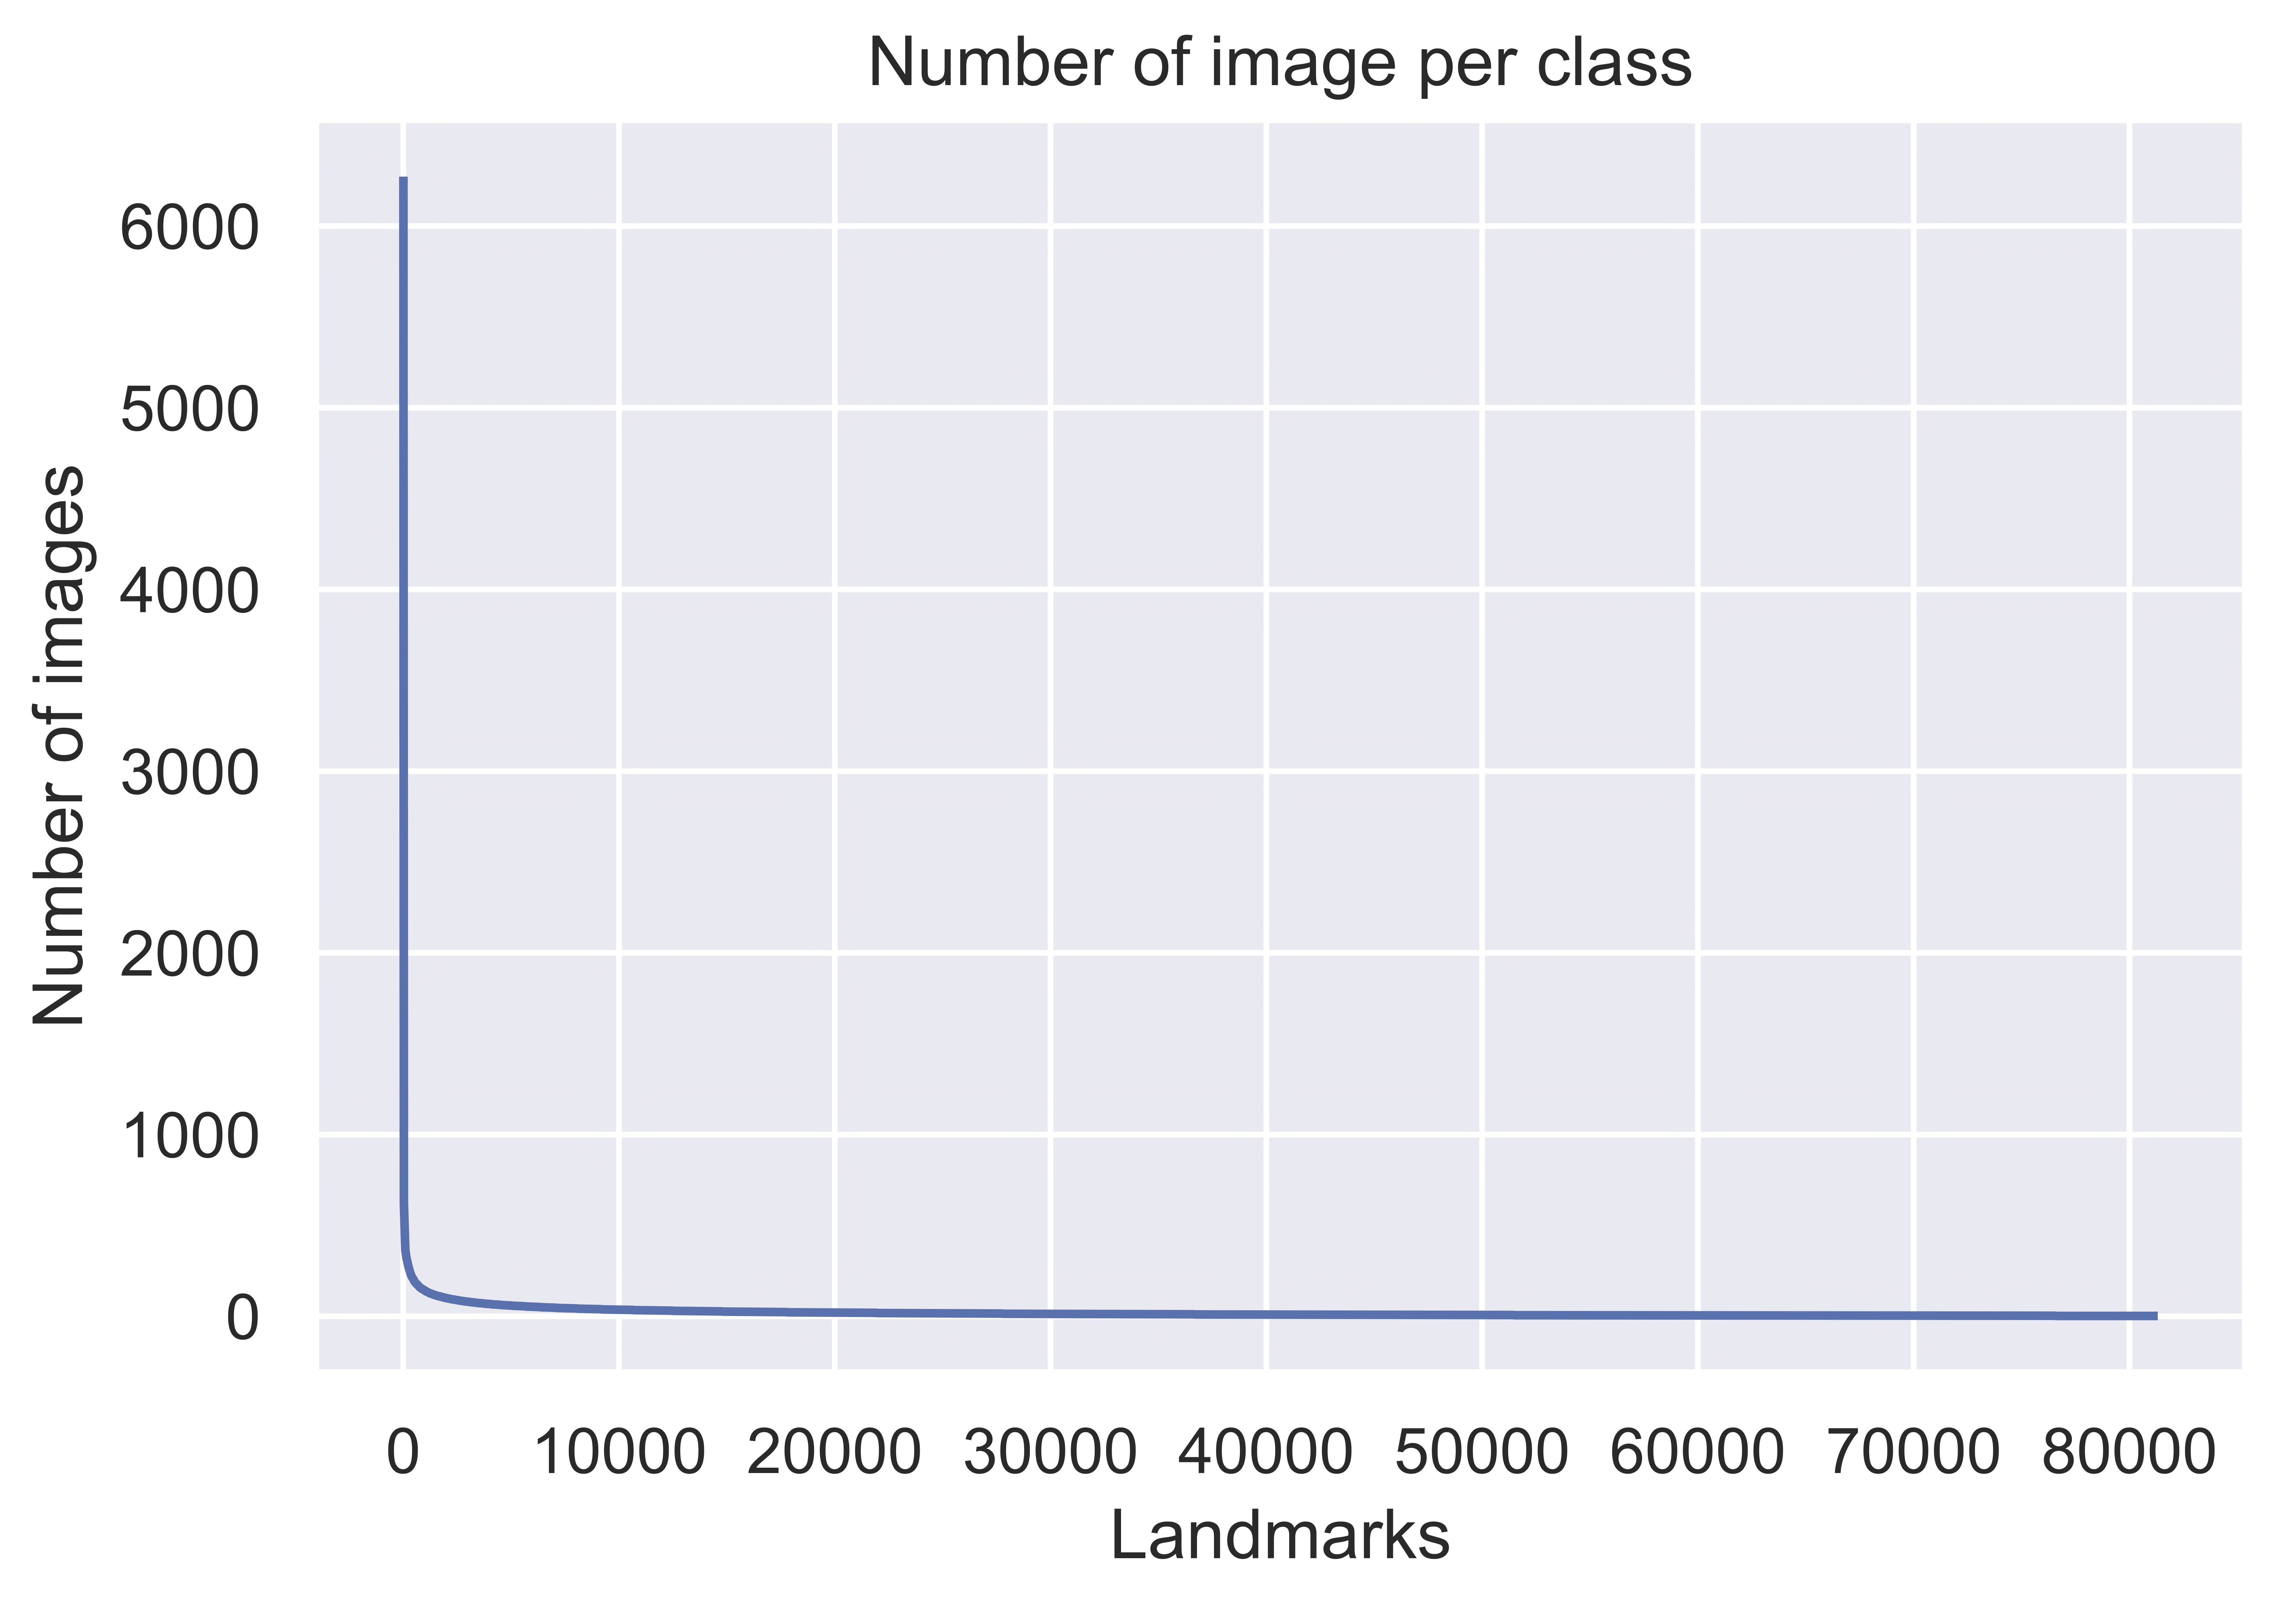
\includegraphics[width=0.5\textwidth]{img/dist.png}
    \caption{Frequency graph of each landmark class. The classes are sorted in descending frequency order.}
    \label{fig:dist_data}
\end{figure}

Besides, the quality of images in the dataset is not very high. There are some quite misleading images even for human beings to recognize. Also, the features in the images from the same landmark class can be very distinct from our visual inspection. Figure \ref{fig:landmark_example} is one of the examples.

\begin{figure}[!htb]
    \centering
    \begin{minipage}[t]{0.23\textwidth}
        \includegraphics[width=\textwidth]{img/4440bfd817bfb6c8.jpg}
    \end{minipage}
    \begin{minipage}[t]{0.23\textwidth}
        \includegraphics[width=\textwidth]{img/1115e27655e0f398.jpg}
    \end{minipage}
    \caption{Example images of the same class in the dataset. The left image can clearly see the landmark where the right image is just a floor plan.}
    \label{fig:landmark_example}
\end{figure}

\subsection{Custom Dataset Creation}
We further create three datasets from this Google landmark dataset. The top 12 and top 20 landmark dataset, which include 12 and 20 landmarks classes with the largest sample size in the original dataset, are first created for preliminary testing. The top 12 landmark dataset has 19999 images while the top 20 landmark dataset has 26779 images. Then, a final dataset is created by discarding all landmark classes with a sample size less than 6. The final dataset has 57042 landmarks classes with 1490153 images in total. All of the datasets are split into training, validation, and test set with the ratio of 0.72, 0.18, 0.1 respectively.

%------------------------------------------------------------------------
\section{Methods}
\subsection{Preprocessing}
In pre-processing, the images are first resize to 224 x 224 in order to fit into the models (ResNet and EfficientNet). Then, apply normalization to the image data. 
To increase the number of data samples for those landmark classes with extremely limited samples, using data augmentation to enlarge their sample size. It also helps reduce the overfitting problem.

%------------------------------------------------------------------------

\subsection{Landmark Recognition Model}
In this project, two deep convolution neural networks, ResNet and EfficientNet are tested and evaluated. Since the dataset is very large, it is time-consuming to train a brand new network due to the limited hardware situation. Therefore, transfer learning technique is applied in order to shorten the training time. The final fully connected layer of the models is replaced with a new fully connected layer with the output size the same as the number of landmarks. Then, the model will be trained for a few epochs.

To further increase the speed of training, both models are trained under mixed precision mode. With proper technique, mixed precision training can speed up the training speed significantly without sacrificing the final model accuracy \cite{micikevicius_mixed_2017}, especially with GPU that has tensor core \cite{noauthor_training_nodate}. For instance, fully connected layers and CNN layers can operate under half-precision (float16) while batch normalization layers can operate in single-precision (float32) in order to reduce the effect of accumulated floating point errors. In addition, mixed precision training also reduce memory usage. Therefore, a larger batch size can be used during training compare with single-precision training with the same size of GPU memory, which also increase the training speed slightly.

In the training progress, two loss functions, cross entropy loss and label-distribution-aware margin (LDAM) Loss\cite{cao_learning_2019} are tested. Cross entropy loss is a very common loss function used in classification problem. It can be considered as a baseline loss function. However, the dataset may have data imbalance issue, which cannot be solved by cross entropy loss. Using this loss function with a extreme imbalance dataset may cause low precision/recall in minority class. To get a better representation on minor class, LDAM loss can be use. The loss function is formulated as such:
\begin{align}
    \mathcal{L}_{LDAM}((x, y); f) &= -\log{\frac{e^{z_y - \Delta_y}}{e^{z_y - \Delta_y} + \sum_{j \ne y}e^{z_j}}}\\
    \text{, }\Delta_j &= \frac{C}{n^{1/4}_j} \textbf{ for } j \in [1,k]
\end{align}
where $C$ is a hyperparameter, $n_j$ is the number of sample of $j$-th class, and $z_j$ is the model prediction output of j-th class. By using LDAM loss, it attempts to increase the margin distance of the minority classes from the decision boundary.

In addition, hyperparameters tuning is required in order to obtain an optimized model. Grid search or Bayesian optimization, which is a more efficient technique, is applied to tune model hyperparameters.

%------------------------------------------------------------------------
\subsection{Evaluation}
To evaluate the performance of the deep learning model, accuracy, precision, recall and F1 score would be used.
\begin{align}
    \textbf{Precision} &= \frac{TP}{TP+FP}\\
    \textbf{Recall} &= \frac{TP}{TP+FN}\\
    \textbf{F1} &= 2 \times \frac{\textbf{Precision} \times \textbf{Recall}}{\textbf{Precision} + \textbf{Recall}}
\end{align}
where $TP$, $TN$, $FP$, $FN$ is the number of true positive, true negative, false positive, false negative prediction of the class respectively. Since the dataset is imbalance, F1 score is consider as a more important evaluation metrics than accuracy. Moreover, confusion matrix would be a visual evaluation metric.

%------------------------------------------------------------------------
\section{Experiments}

\subsection{Experiment Environment and Implementation}
The computer we used for the model training has an 8-core CPU with Nvidia GeForce RTX 2070 Super. The operating system is Ubuntu 18.04 LTS.

All codes are implemented in Python 3.7.9, and the models are implemented with \href{https://pytorch.org/}{PyTorch} \cite{paszke_pytorch_2019} along with some common python packages, such as \href{https://numpy.org/}{Numpy}, \href{https://pandas.pydata.org/}{Pandas}, and \href{https://scikit-learn.org/}{scikit-learn}. The ResNet50 pretrained model are retrieved from \href{https://pytorch.org/docs/stable/torchvision/index.html}{torchvision} library, and the EfficientNet-B0 pretrained model are retrieved from a python package EfficientNet\_PyTorch\footnote{https://github.com/lukemelas/EfficientNet-PyTorch}. Also, python package \href{https://ax.dev/}{Ax} are used for hyperparameter optimizaiton.

%------------------------------------------------------------------------

\subsection{Experiment}
Before implementing the model on the whole dataset, top 12 and top 20 landmark classes is first selected to do some experiments. Each sub dataset is split into three parts: training, validation, and testing with the ratio of 0.72, 0.18, 0.1. For both datasets, using ResNet50 and EfficientNet-B0 as training models and cross-entropy as loss function.

From the performance of these two sub-datasets(table \ref{tab:table1} and table \ref{tab:table2}), we can observe that as more landmark classes are in the dataset, the accuracy will decrease. The main reason is that the minority class has relatively low precision and recall. As shown in the confusion matrix in figure \ref{fig:cm_top20}, the images of landmarks with fewer samples are misclassified as some other landmarks with much more sample. This is a common issue in model training with an imbalanced dataset. Therefore, to cope with the dataset with more landmarks and more severe imbalance issues, LDAM is implemented to resolve this issue. 

After implementing the LDAM as loss function for the top 20 landmark classes dataset, the model performance has improved as both training and testing accuracy increase as shown in table \ref{tab:table2}. Therefore, the LDAM loss function will be applied to the later big dataset.

\begin{table}[]
    \centering
    \begin{tabular}{c c c}
        \hline Model & Training Acc & Testing Acc \\ \hline
        ResNet50 & $98.02\%$ & $96.65\%$ \\
        EfficientNet-B0 & $97.69\%$ & $98.05\%$ \\ \hline
    \end{tabular}
    \vspace{5pt}
    \caption{Model performance of top 12 landmark classes dataset}
    \label{tab:table1}
\end{table}

\begin{table*}
    \centering
    \begin{tabular}{c c c c}
        \hline Model & Training Accuracy & Testing Accuracy & Testing Average F1 \\ \hline
        ResNet50 & $96.05\%$ & $94\%$ & $0.92$ \\
        ResNet50+LDAM & $97.88\%$ & $94.18\%$ & $0.95$ \\
        EfficientNet-B0 & $92.40\%$ & $92.72\%$ & $0.91$ \\ 
        EfficientNet-B0+LDAM & $99.48\%$ & $98.02\%$ & $0.97$ \\ \hline
    \end{tabular}
    \vspace{5pt}
    \caption{Model performance of top 20 landmark classes dataset}
    \label{tab:table2}
\end{table*}

\begin{figure}
    \centering
    \begin{minipage}[t]{0.4\textwidth}
        \includegraphics[width=\textwidth]{COMP4471_Final_Report/img/top20_test_resnet.png}
    \end{minipage}
    \begin{minipage}[t]{0.4\textwidth}
        \includegraphics[width=\textwidth]{COMP4471_Final_Report/img/top20_test_efficientnet.png}
    \end{minipage}
    \caption{Test set confusion matrix of top-20 landmark classification with ResNet50(top) and EfficientNet-B0(bottom). The larger the landmark id, the fewer the sample that landmark have}
    \label{fig:cm_top20}
\end{figure}

From the original training dataset with $81313$ landmark classes, discard those classes with a number of images less than six. After that, there are finally $57042$ landmark classes with $1490153$ images in total. This dataset is also split into three parts: training, validation, and testing with the ratio of 0.72, 0.18, 0.1. Data augmentations with some random flipping and color jittering are used on the training data in order to mitigate the effect of the imbalanced dataset issue. Because the dataset is quite large (over one million images for training dataset), methods to speed up the training process under limited resources are in need. First of all, resize all the images to store in the size of $224$x$224$. Due to the limited RAM, each batch of data is loaded while training the model instead of loading all the data beforehand. Mixed precision training is applied in order to reduce the networks' runtime and memory footprint, since some operations, like linear layers and convolutions, can be much faster in float16 (half) datatype. Also, add gradient scaling to prevent gradients with small magnitudes from vanishing under mixed precision training.

\begin{table*}[]
    \centering
    \begin{tabular}{c c c c}
        \hline Model & Training Accuracy & Testing Accuracy & Testing Average F1 \\ \hline
        ResNet50+LDAM & $80.26\%$ & $67.70\%$ & 0.60 \\
        EfficientNet-B0+LDAM & $76.98\%$ & $68.19\%$ & 0.61 \\ \hline
    \end{tabular}
    \vspace{5pt}
    \caption{Model performance of 57042 landmark classes dataset}
    \label{tab:table3}
\end{table*}

\begin{figure}
    \centering
    % \begin{minipage}[t]{0.23\textwidth}
    %     \includegraphics[width=\textwidth]{img/resnet_f1_dist.png}
    % \end{minipage}
    \begin{minipage}[t]{0.4\textwidth}
        \includegraphics[width=\textwidth]{COMP4471_Final_Report/img/resent_f1_dist.png}
    \end{minipage}
    \begin{minipage}[t]{0.4\textwidth}
        \includegraphics[width=\textwidth]{COMP4471_Final_Report/img/efficientnet_f1_dist.png}
    \end{minipage}
    \caption{F1 score histogram of ResNet50(top) and EfficientNet-B0(bottom)}
    \label{fig:f1_dist}
\end{figure}

The final training results are shown in table \ref{tab:table3}. The testing performances of the two networks drop a lot as the number of landmark classes is extremely large. Analyzing the f1 scores of each network, both models have over $20000$ classes with f1 score over 0.9 and around $15000$ classes with f1 score lower than 0.1 as shown in the F1 score histograms in figure \ref{fig:f1_dist}. Most of the landmark classes with f1 score lower than 0.1 are minority classes with just a few samples in the test set, and hence the support of these f1 score is very small. Having a further look into the f1 scores, we found that there are some landmarks classes with relatively large size datasets getting very low f1 scores. For instance, landmark 177870 has $783$ samples for training, however, in both EfficientNet and ResNet model, its f1 scores are $0.215$ and $0.3968$ respectively. From figure \ref{fig:class_177870}, it quite obvious that the architectural styles of these four buildings are very different, which indicates the dataset quality of this class is not good and it seems that the prediction performance is also influenced by this low quality of the dataset. As for landmark class $169630$ which has only 4 images for training, but the testing f1 scores of both models are 1. From (figure \ref{fig:class_169630}), it can be easily observed that these four images are the same landmark as the feature of this class is presented very well, which can be inferred that the quality of this class samples is quite high.

\begin{figure}[]
    \centering
    \begin{minipage}[t]{0.23\textwidth}
        \includegraphics[width=\textwidth]{COMP4471_Final_Report/img/177870_01.png}
    \end{minipage}
    \begin{minipage}[t]{0.23\textwidth}
        \includegraphics[width=\textwidth]{COMP4471_Final_Report/img/177870_02.png}
    \end{minipage}
    \begin{minipage}[t]{0.23\textwidth}
        \includegraphics[width=\textwidth]{COMP4471_Final_Report/img/177870_03.png}
    \end{minipage}
    \begin{minipage}[t]{0.23\textwidth}
        \includegraphics[width=\textwidth]{COMP4471_Final_Report/img/177870_04.png}
    \end{minipage}
    \caption{Example images of the class 177870 in the dataset.}
    \label{fig:class_177870}
\end{figure}

\begin{figure}[]
    \centering
    \begin{minipage}[t]{0.23\textwidth}
        \includegraphics[width=\textwidth]{COMP4471_Final_Report/img/169630_01.png}
    \end{minipage}
    \begin{minipage}[t]{0.23\textwidth}
        \includegraphics[width=\textwidth]{COMP4471_Final_Report/img/169630_02.png}
    \end{minipage}
    \begin{minipage}[t]{0.23\textwidth}
        \includegraphics[width=\textwidth]{COMP4471_Final_Report/img/169630_03.png}
    \end{minipage}
    \begin{minipage}[t]{0.23\textwidth}
        \includegraphics[width=\textwidth]{COMP4471_Final_Report/img/169630_04.png}
    \end{minipage}
    \caption{Example images of the class 169630 in the dataset.}
    \label{fig:class_169630}
\end{figure}

%------------------------------------------------------------------------
\section{Conclusion}
From the experiment result, both ResNet50 and EfficientNet-B0 achieve accuracy of over 65\% and average F1 score over 0.50. LDAM loss indeed improves the performance of both models. However, since the dataset is extremely imbalanced, the effect of LDAM loss on the model performance is limited and models still perform poorly in minority classes.

Both models have similar performance in terms of accuracy and F1 score. However, the parameter size of the two models is very different. ResNet50 has over 25 million parameters while EfficientNet-B0 only has about 5 million parameters. EfficientNet-B0 can achieve similar performance with way fewer parameters than ResNet50. Thus, we consider EfficientNet-B0 as the best model for landmark recognition.

% \clearpage
{\small
\bibliographystyle{ieee}
\bibliography{egbib}
}

\end{document}
